\subsection{Input rescaling and prediction error}
Both raw-input kernels are fitted at five nested
training sizes over a sixteenfold range, at ten seeds on each band.
Each sensitivity map is estimated from the training rows available at its
own sample size using the standardized-input least-squares matrix $A$ in
Supplement~\ref{supp:oco-input}. Rank summaries use the separate matrix
$B=X_{\rm tr}^{\dagger}Z$ in the released input coordinates on all 18000
fitting rows. The singular-value counts retaining $99\%$ of $B$'s squared
energy are $12/20$, $14/24$ and $13/24$; the corresponding participation
ratios $(\sum_j\sigma_j)^2/\sum_j\sigma_j^2$ are $11.99$, $13.63$ and
$13.33$. These describe the fitted linear maps in those coordinates.

Table~\ref{tab:aniso} reports finite-range log--log slopes. On O2 the paired
slope difference is small relative to its seed variation. The adapted
kernel's fitted exponent is larger on the two CO$_2$ bands, by $0.011$ and
$0.052$. At $n=18000$ the isotropic-to-adapted error ratios are
$1.353\pm0.008$, $1.118\pm0.002$ and $1.514\pm0.114$. Thus the tested
rescaling improves prediction at that training size but leaves much of
the error difference between raw-input and feature kernels. These finite-range slopes are distinct from the rank-truncation bound of
Proposition~\ref{prop:aniso}, which requires Lipschitz, domain-radius, and
native-space assumptions beyond the estimated ranks.

\begin{table}[t]
\centering
\caption{The raw-input kernel refit at nested training sizes, ten seeds per
band. ``Rank'' counts singular values of the fitting-set matrix $B=X_{\rm tr}^{\dagger}Z$
holding $99\%$ of the squared energy, out of the input dimension. The exponent
difference is paired within seed; its standard deviation is over seeds. The
last column is the isotropic-to-adapted error ratio at $n=18000$.
The slopes are descriptive fits over the finite sizes tested.}
\label{tab:aniso}
\begin{adjustbox}{max width=\linewidth}
\begin{tabular}{lccccc}
\toprule
Band & Rank & $-$slope iso & $-$slope adapted & difference & ratio at $n{=}18000$ \\
\midrule
O2         & 12/20 & $0.221\pm0.007$ & $0.215\pm0.017$ & $+0.006\pm0.015$ & $1.353\pm0.008$ \\
weak CO$_2$   & 14/24 & $0.086\pm0.005$ & $0.097\pm0.006$ & $-0.011\pm0.009$ & $1.118\pm0.002$ \\
strong CO$_2$ & 13/24 & $0.203\pm0.029$ & $0.255\pm0.020$ & $-0.052\pm0.021$ & $1.514\pm0.114$ \\
\bottomrule
\end{tabular}
\end{adjustbox}
\end{table}

At $n=18000$, the sweep and Table~\ref{tab:oco2} use the same tuning
routine and standardized inputs and give identical raw-kernel results and
selected hyperparameters at every seed.
Training duration affects the comparison: a separate single-seed
$750$-epoch O2 run reaches $3.82\%$ (flat network)
and $3.71\%$ (feature head), with the combination at $3.71\%$ reduced and $0.0174\%$
radiance. The $250$-epoch comparison is therefore sensitive to training
duration and does not establish convergence.

The training-loss comparison further distinguishes coordinate
weighting from per-case weighting. The second network in
Table~\ref{tab:oco2} is trained on a diagonally weighted loss over the
reduced coefficients, $\|s_z\odot(\hat z-z)\|/\|s_z\odot z\|$. That is a surrogate for the radiance-relative error: the reported radiance metric maps predictions through the stored PCA
reconstruction and divides by the reconstructed-radiance norm, and the
surrogate omits the reconstruction. The third network is trained in the
exact radiance metric, reconstruction and denominator included. Its
radiance error is higher than that of the surrogate-trained network:
$0.0571\pm0.0057\%$ against $0.0442\pm0.0044\%$ on O2
and $0.093\pm0.008\%$ against $0.075\pm0.003\%$ on SCO2, the surrogate having lower error at all ten seeds on both bands. The
ranking is reversed on WCO2 at eight of ten seeds
($0.064\pm0.015\%$ against $0.072\pm0.007\%$). The kernel heads built on
their features repeat the pattern. Tripling the training budget narrows the
O2 gap ($0.0212\%$ against $0.0201\%$ at $750$ epochs) without reversing it,
but these finite-budget comparisons do not identify why one training loss
performs better. By the reconstruction identity, the two losses share the
same numerator and differ in their target-dependent denominator, which
reweights cases. Both concentrate on the leading coefficients, while their
optimization and generalization behavior can differ. The coordinate
profile is consistent with this trade-off: the kernel-flow emulator
predicts the leading coefficient to $0.0012$ root mean square against the
flat network's $0.0054$, whereas the flat network is three to four times
more accurate on the trailing thirty coordinates. The relative errors depend on both the band and training budget.

The flat-network seeds permit a second-moment analysis similar to
that on structural mechanics.
For each band, the matrix $S$ contains the test-set second moments of the
normalized residuals of the ten flat-network seeds. Mixture risks are
measured in squared relative error, as in Proposition~\ref{prop:secmom}.

At uniform weights, $w^\top Sw$ and the
directly measured risk of the averaged prediction agree to $7\times10^{-18}$,
$3\times10^{-17}$ and $1\times10^{-17}$ on the three bands.

Over the $45$ seed pairs per band, the residual alignments are
$0.787\pm0.010$ (O2), $0.971\pm0.001$ (WCO2) and
$0.961\pm0.001$ (SCO2). An equicorrelation summary gives ten-member RMS
relative errors of $4.419\%$, $17.997\%$ and $9.267\%$, matching the
recorded uniform-mixture risks at the displayed precision. The corresponding
infinite-family values, $4.360\%$, $17.970\%$ and $9.248\%$, are
extrapolations under the equicorrelation model. They are not lower bounds
for untrained seeds or for the architecture class. The exact
finite-pool statement is the quadratic identity applied to the measured
matrix $S$.

Comparisons with another readout must use the same metric, since $S$
determines a squared-relative-error quantity and
Table~\ref{tab:oco2} reports the mean relative error $\mathbb E\,\ell$.
Measured in RMS relative error, the Mat\'ern head on learned
features reaches $4.575\%$, $18.11\%$ and $9.326\%$ --- better than an
individual seeded network ($4.915\%$, $18.238\%$, $9.433\%$) and worse than
that network's ten-seed ensemble. The ranking is the same in the mean metric,
where the seed ensemble reaches $3.916\%$ against the head's $4.111\%$ on
O2. The ten-network ensemble has lower error than the single feature-kernel
head in both metrics, but the predictors have different computational costs.

Lower residual alignment alone does not guarantee a useful mixture: the
weaker member's RMS error also enters Proposition~\ref{prop:secmom}(i).
An exploratory WCO2 Fourier-feature bandwidth sweep gives error near
$31\%$ with correlation $0.54$, and errors above $140\%$ with correlations
near $0.11$ (Figure~\ref{fig:floor}). The plotted errors and correlations
are rounded summaries; the admission-condition analysis in
Section~\ref{sec:secmom-margin} uses the exact uncentered second moments
of the eight-model pool.
Adding the exploratory architecture candidates
to coordinate selection changed the mean error by less than $0.01$
percentage points on each band.

\begin{figure}[t]
\centering
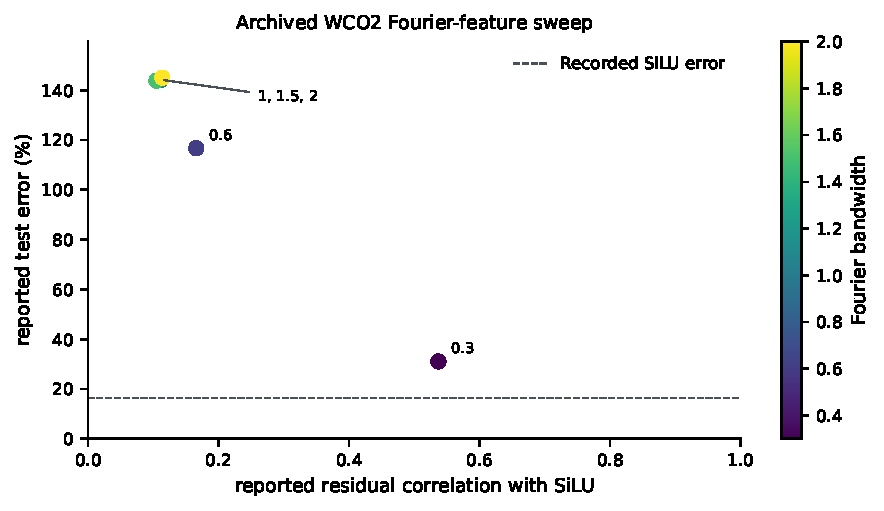
\includegraphics[width=\linewidth]{figs/floor.pdf}
\caption{Exploratory WCO2 Fourier-feature sweep. The legend identifies bandwidths; the
dashed line is the SiLU error of $16.37\%$. Three bandwidths nearly
coincide in the upper left. Errors and correlations are rounded
summaries of the exploratory measurements. The admission calculations in
Section~\ref{sec:secmom-margin} use exact uncentered second moments.}
\label{fig:floor}
\end{figure}

For the raw-input kernel against the flat network, the validation
summary has $\varrho=0.156$ and $e_n/e_k=0.157$, with RMS relative errors
$8.41\%$ and $53.5\%$. The sign of the criterion changes across seeds,
and the optimal mixture gains only a few ten-thousandths of a
percentage point. This explains the pair's small
contribution.

The combination chooses each coordinate from one of the three networks
and three feature-kernel heads using coordinatewise validation RMSE. By
Proposition~\ref{prop:percoord}, this minimizes an auxiliary separable
squared loss over that candidate product. Fixed sample denominators retain
separability for squared relative losses, with different sample weights
for the reduced and radiance criteria. The reported means of relative
norms instead couple coordinates through the square root. Consequently
this selector is not guaranteed to optimize either reported metric, or
both simultaneously. The same selected coordinates produce both reported
columns; the baseline emulator's predictions are not candidates.
Its seed-averaged errors are lower than those of the rescored
kernel-flow emulator in both criteria on all three bands: O2 reaches
$4.12\pm0.05\%$ against $16.89\%$ reduced and $0.0294\pm0.0020\%$ against
$0.0448\%$ radiance, SCO2 $8.08\pm0.01\%$ against $16.14\%$ and
$0.0584\pm0.0041\%$ against $0.1147\%$, and WCO2 $16.28\pm0.06\%$ against
$24.06\%$ and $0.0507\pm0.0052\%$ against $0.0599\%$. Counted by seed, the
combination has lower error than the emulator in both metrics at all ten
seeds on O2 and SCO2 and at nine of ten on WCO2. At the remaining WCO2 seed,
its radiance error is higher by $0.0015$ percentage points.

On O2 the combination's reduced mean is slightly worse than that of the
flat-feature head ($4.11510\%$ versus $4.11080\%$), while its radiance mean
improves from $0.07927\%$ to $0.02940\%$. The selector therefore improves radiance accuracy at a small cost in
reduced-coordinate accuracy. On WCO2, one seed has a radiance error
$0.0015$ percentage points higher than the source emulator. The paired-bootstrap interval for that seed is
$[-0.0012,0.0042]$ percentage points, while the other nine intervals are
negative. These are descriptive intervals on the public test cases.

\subsection{Learning curves and training budgets}
\label{sec:scaling}
The OCO-2 learning curve decreases more strongly with training
size than the structural-mechanics curve over the ranges examined.
The left panel of Figure~\ref{fig:ocoscaling} shows a one-seed O2 experiment
with a disjoint held-out set. A finite-range log--log fit gives slope
$-0.68$, with error decreasing from about $74\%$ at a few hundred pairs to
$4.3\%$ at $n=17700$. The main ten-seed combination at $18000$ training
pairs has mean $4.12\%$ at its $250$-epoch budget; the $3.71\%$ result
above belongs to a separate single-seed $750$-epoch experiment. These are
different protocols and should not be combined into one scaling fit.
The raw-input kernel improves more slowly over these sizes. The measured
curves do not identify the limiting source of error or an asymptotic
convergence rate.

The ClimSim experiments cover a larger data range. ClimSim \citep{yu2023climsim} is a climate emulation dataset of about
ten million samples that maps a $124$-dimensional atmospheric state to $128$
physics tendencies, with published neural baselines. The runs compare two model
families at one, two and three and a half million training samples.
Kernel hyperparameters are selected on a disjoint 2000-row validation
block drawn from the training pool. Each neural run retains the final
checkpoint of its 60-epoch schedule. Evaluation uses separate data; the
right panel of Figure~\ref{fig:ocoscaling} plots those points. Each experiment
seed draws its own $20000$-row test block, so the spreads below include that
variation.

For each output coordinate $j$, let
$v_j=N^{-1}\sum_{i=1}^N(y_{ij}-\bar y_j)^2+10^{-12}$ be its variance
on that seed's test block, and define
$J=\{j:v_j>10^{-6}\max_k v_k\}$. The reported score is the unweighted
mean of the coordinatewise coefficients of determination,
\[
 R^2=\frac{1}{|J|}\sum_{j\in J}
 \left(1-\frac{N^{-1}\sum_{i=1}^N(\hat y_{ij}-y_{ij})^2}{v_j}\right).
\]
The same active-coordinate set $J$ is used for both predictors at each seed.

The neural mean has higher $R^2$ than the kernel and improves with training
size: $0.544\pm0.005$ at one
million (five seeds), $0.563\pm0.004$ at two million and $0.575\pm0.004$ at
three and a half million (three seeds each). A published
multilayer-perceptron value near $0.6$ provides context; this comparison
does not use a matched split and scoring protocol. The corresponding kernel values are $0.390\pm0.007$, $0.391\pm0.006$ and $0.387\pm0.007$ at the three
sizes. Each kernel was fitted on a $6000$-row subsample, so the near-constant
error does not describe its response to increasing kernel training size.
A separate kernel-budget comparison uses the same protocol
(selection on the pool validation block, separate test evaluation, seed
$0$, the one-million slice): $\csCapSix$ at $6000$ rows, $\csCapTwelve$ at
$12000$ and $\csCapTwentyFour$ at $24000$ ($\csCapTwentyFourB$ at a second
seed, with a separately drawn test block). The $R^2$ value increases by about $0.03$ at the first budget doubling
and $0.01$ at the second, and at
$24000$ rows, the largest exact solve tested, its $R^2$ remains about $0.11$
below the network at
one million samples. The comparison remains unequal in training size and total computation:
the neural mean uses up to millions of examples, whereas the exact kernel
uses at most $24000$. The network has lower error under these budgets; matched-compute
comparisons and larger kernel fits remain untested. The reported range does not locate a
crossover between model families.

\begin{figure}[t]
\centering
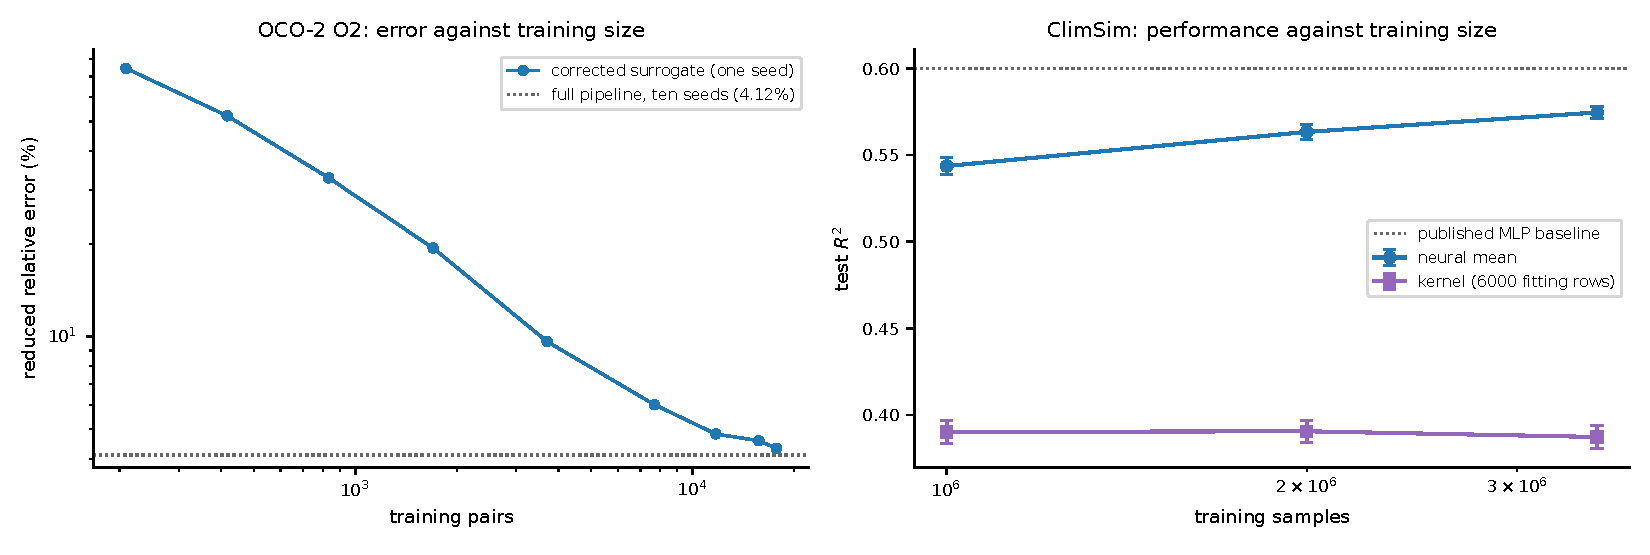
\includegraphics[width=\linewidth]{figs/scaling_seeded.pdf}
\caption{Error against training-set size. Left: the
OCO-2 O2 task, reduced error of the corrected surrogate at one seed, from the
data-scaling run; a finite-range log--log fit has slope $-0.68$, and the
error is $4.3\%$ at $n=17700$, against the
$4.12\%$ the ten-seed pipeline reaches on all $18000$ pairs (dotted). Right:
ClimSim, test $R^2$ over the active outputs defined in the text, at one,
two and three and a half million training samples --- five seeds at one million and three at each of the
larger sizes, error bars over seeds. No crossover between the two families is observed over this range. Each kernel is fitted on $6000$ rows, so its nearly constant error
across nominal training sizes reflects that fixed fitting budget. The separate
kernel-budget comparison is reported in the text. The neural
mean has higher $R^2$; the published baseline (dotted) is shown for orientation; the protocols are not matched.}
\label{fig:ocoscaling}
\end{figure}
